% Created by tikzDevice version 0.12.3.1 on 2022-05-11 23:38:56
% !TEX encoding = UTF-8 Unicode
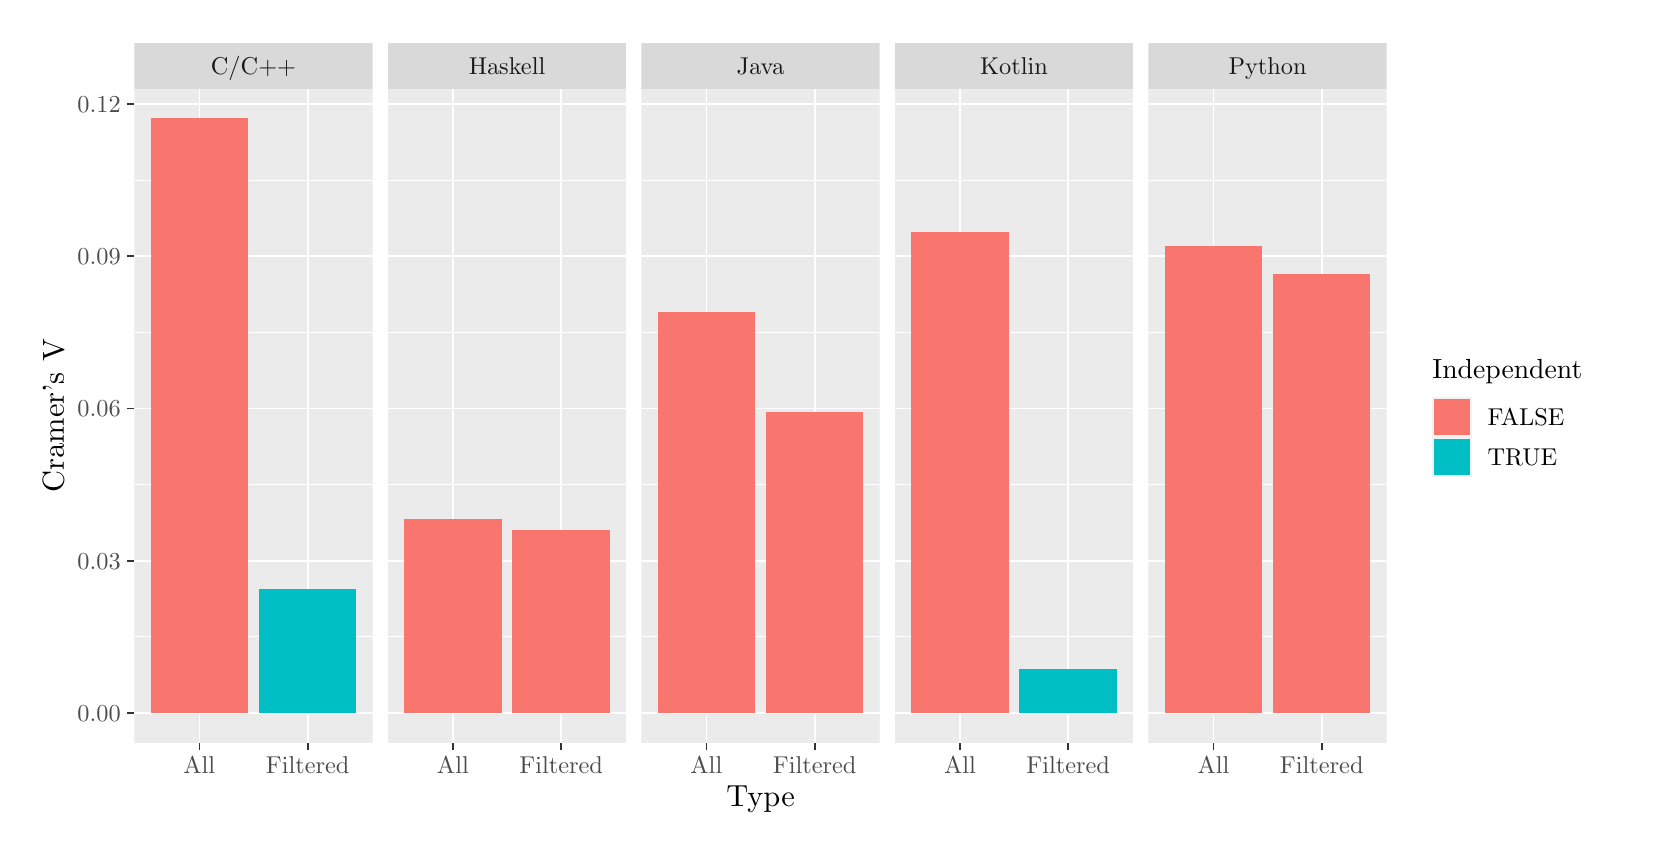
\begin{tikzpicture}[x=1pt,y=1pt]
\definecolor{fillColor}{RGB}{255,255,255}
\path[use as bounding box,fill=fillColor,fill opacity=0.00] (0,0) rectangle (578.16,289.08);
\begin{scope}
\path[clip] (  0.00,  0.00) rectangle (578.16,289.08);
\definecolor{drawColor}{RGB}{255,255,255}
\definecolor{fillColor}{RGB}{255,255,255}

\path[draw=drawColor,line width= 0.6pt,line join=round,line cap=round,fill=fillColor] (  0.00,  0.00) rectangle (578.16,289.08);
\end{scope}
\begin{scope}
\path[clip] ( 38.56, 30.69) rectangle (124.66,267.01);
\definecolor{fillColor}{gray}{0.92}

\path[fill=fillColor] ( 38.56, 30.69) rectangle (124.66,267.01);
\definecolor{drawColor}{RGB}{255,255,255}

\path[draw=drawColor,line width= 0.3pt,line join=round] ( 38.56, 68.94) --
	(124.66, 68.94);

\path[draw=drawColor,line width= 0.3pt,line join=round] ( 38.56,123.95) --
	(124.66,123.95);

\path[draw=drawColor,line width= 0.3pt,line join=round] ( 38.56,178.97) --
	(124.66,178.97);

\path[draw=drawColor,line width= 0.3pt,line join=round] ( 38.56,233.98) --
	(124.66,233.98);

\path[draw=drawColor,line width= 0.6pt,line join=round] ( 38.56, 41.43) --
	(124.66, 41.43);

\path[draw=drawColor,line width= 0.6pt,line join=round] ( 38.56, 96.44) --
	(124.66, 96.44);

\path[draw=drawColor,line width= 0.6pt,line join=round] ( 38.56,151.46) --
	(124.66,151.46);

\path[draw=drawColor,line width= 0.6pt,line join=round] ( 38.56,206.47) --
	(124.66,206.47);

\path[draw=drawColor,line width= 0.6pt,line join=round] ( 38.56,261.49) --
	(124.66,261.49);

\path[draw=drawColor,line width= 0.6pt,line join=round] ( 62.04, 30.69) --
	( 62.04,267.01);

\path[draw=drawColor,line width= 0.6pt,line join=round] (101.18, 30.69) --
	(101.18,267.01);
\definecolor{fillColor}{RGB}{248,118,109}

\path[fill=fillColor] ( 44.43, 41.43) rectangle ( 79.65,256.27);
\definecolor{fillColor}{RGB}{0,191,196}

\path[fill=fillColor] ( 83.57, 41.43) rectangle (118.79, 86.28);
\end{scope}
\begin{scope}
\path[clip] (130.16, 30.69) rectangle (216.27,267.01);
\definecolor{fillColor}{gray}{0.92}

\path[fill=fillColor] (130.16, 30.69) rectangle (216.27,267.01);
\definecolor{drawColor}{RGB}{255,255,255}

\path[draw=drawColor,line width= 0.3pt,line join=round] (130.16, 68.94) --
	(216.27, 68.94);

\path[draw=drawColor,line width= 0.3pt,line join=round] (130.16,123.95) --
	(216.27,123.95);

\path[draw=drawColor,line width= 0.3pt,line join=round] (130.16,178.97) --
	(216.27,178.97);

\path[draw=drawColor,line width= 0.3pt,line join=round] (130.16,233.98) --
	(216.27,233.98);

\path[draw=drawColor,line width= 0.6pt,line join=round] (130.16, 41.43) --
	(216.27, 41.43);

\path[draw=drawColor,line width= 0.6pt,line join=round] (130.16, 96.44) --
	(216.27, 96.44);

\path[draw=drawColor,line width= 0.6pt,line join=round] (130.16,151.46) --
	(216.27,151.46);

\path[draw=drawColor,line width= 0.6pt,line join=round] (130.16,206.47) --
	(216.27,206.47);

\path[draw=drawColor,line width= 0.6pt,line join=round] (130.16,261.49) --
	(216.27,261.49);

\path[draw=drawColor,line width= 0.6pt,line join=round] (153.65, 30.69) --
	(153.65,267.01);

\path[draw=drawColor,line width= 0.6pt,line join=round] (192.79, 30.69) --
	(192.79,267.01);
\definecolor{fillColor}{RGB}{248,118,109}

\path[fill=fillColor] (136.03, 41.43) rectangle (171.26,111.54);

\path[fill=fillColor] (175.17, 41.43) rectangle (210.40,107.68);
\end{scope}
\begin{scope}
\path[clip] (221.77, 30.69) rectangle (307.88,267.01);
\definecolor{fillColor}{gray}{0.92}

\path[fill=fillColor] (221.77, 30.69) rectangle (307.88,267.01);
\definecolor{drawColor}{RGB}{255,255,255}

\path[draw=drawColor,line width= 0.3pt,line join=round] (221.77, 68.94) --
	(307.88, 68.94);

\path[draw=drawColor,line width= 0.3pt,line join=round] (221.77,123.95) --
	(307.88,123.95);

\path[draw=drawColor,line width= 0.3pt,line join=round] (221.77,178.97) --
	(307.88,178.97);

\path[draw=drawColor,line width= 0.3pt,line join=round] (221.77,233.98) --
	(307.88,233.98);

\path[draw=drawColor,line width= 0.6pt,line join=round] (221.77, 41.43) --
	(307.88, 41.43);

\path[draw=drawColor,line width= 0.6pt,line join=round] (221.77, 96.44) --
	(307.88, 96.44);

\path[draw=drawColor,line width= 0.6pt,line join=round] (221.77,151.46) --
	(307.88,151.46);

\path[draw=drawColor,line width= 0.6pt,line join=round] (221.77,206.47) --
	(307.88,206.47);

\path[draw=drawColor,line width= 0.6pt,line join=round] (221.77,261.49) --
	(307.88,261.49);

\path[draw=drawColor,line width= 0.6pt,line join=round] (245.25, 30.69) --
	(245.25,267.01);

\path[draw=drawColor,line width= 0.6pt,line join=round] (284.39, 30.69) --
	(284.39,267.01);
\definecolor{fillColor}{RGB}{248,118,109}

\path[fill=fillColor] (227.64, 41.43) rectangle (262.87,186.41);

\path[fill=fillColor] (266.78, 41.43) rectangle (302.01,150.29);
\end{scope}
\begin{scope}
\path[clip] (313.38, 30.69) rectangle (399.48,267.01);
\definecolor{fillColor}{gray}{0.92}

\path[fill=fillColor] (313.38, 30.69) rectangle (399.48,267.01);
\definecolor{drawColor}{RGB}{255,255,255}

\path[draw=drawColor,line width= 0.3pt,line join=round] (313.38, 68.94) --
	(399.48, 68.94);

\path[draw=drawColor,line width= 0.3pt,line join=round] (313.38,123.95) --
	(399.48,123.95);

\path[draw=drawColor,line width= 0.3pt,line join=round] (313.38,178.97) --
	(399.48,178.97);

\path[draw=drawColor,line width= 0.3pt,line join=round] (313.38,233.98) --
	(399.48,233.98);

\path[draw=drawColor,line width= 0.6pt,line join=round] (313.38, 41.43) --
	(399.48, 41.43);

\path[draw=drawColor,line width= 0.6pt,line join=round] (313.38, 96.44) --
	(399.48, 96.44);

\path[draw=drawColor,line width= 0.6pt,line join=round] (313.38,151.46) --
	(399.48,151.46);

\path[draw=drawColor,line width= 0.6pt,line join=round] (313.38,206.47) --
	(399.48,206.47);

\path[draw=drawColor,line width= 0.6pt,line join=round] (313.38,261.49) --
	(399.48,261.49);

\path[draw=drawColor,line width= 0.6pt,line join=round] (336.86, 30.69) --
	(336.86,267.01);

\path[draw=drawColor,line width= 0.6pt,line join=round] (376.00, 30.69) --
	(376.00,267.01);
\definecolor{fillColor}{RGB}{248,118,109}

\path[fill=fillColor] (319.25, 41.43) rectangle (354.47,215.31);
\definecolor{fillColor}{RGB}{0,191,196}

\path[fill=fillColor] (358.39, 41.43) rectangle (393.61, 57.44);
\end{scope}
\begin{scope}
\path[clip] (404.98, 30.69) rectangle (491.09,267.01);
\definecolor{fillColor}{gray}{0.92}

\path[fill=fillColor] (404.98, 30.69) rectangle (491.09,267.01);
\definecolor{drawColor}{RGB}{255,255,255}

\path[draw=drawColor,line width= 0.3pt,line join=round] (404.98, 68.94) --
	(491.09, 68.94);

\path[draw=drawColor,line width= 0.3pt,line join=round] (404.98,123.95) --
	(491.09,123.95);

\path[draw=drawColor,line width= 0.3pt,line join=round] (404.98,178.97) --
	(491.09,178.97);

\path[draw=drawColor,line width= 0.3pt,line join=round] (404.98,233.98) --
	(491.09,233.98);

\path[draw=drawColor,line width= 0.6pt,line join=round] (404.98, 41.43) --
	(491.09, 41.43);

\path[draw=drawColor,line width= 0.6pt,line join=round] (404.98, 96.44) --
	(491.09, 96.44);

\path[draw=drawColor,line width= 0.6pt,line join=round] (404.98,151.46) --
	(491.09,151.46);

\path[draw=drawColor,line width= 0.6pt,line join=round] (404.98,206.47) --
	(491.09,206.47);

\path[draw=drawColor,line width= 0.6pt,line join=round] (404.98,261.49) --
	(491.09,261.49);

\path[draw=drawColor,line width= 0.6pt,line join=round] (428.47, 30.69) --
	(428.47,267.01);

\path[draw=drawColor,line width= 0.6pt,line join=round] (467.61, 30.69) --
	(467.61,267.01);
\definecolor{fillColor}{RGB}{248,118,109}

\path[fill=fillColor] (410.85, 41.43) rectangle (446.08,210.15);

\path[fill=fillColor] (449.99, 41.43) rectangle (485.22,200.15);
\end{scope}
\begin{scope}
\path[clip] ( 38.56,267.01) rectangle (124.66,283.58);
\definecolor{fillColor}{gray}{0.85}

\path[fill=fillColor] ( 38.56,267.01) rectangle (124.66,283.58);
\definecolor{drawColor}{gray}{0.10}

\node[text=drawColor,anchor=base,inner sep=0pt, outer sep=0pt, scale=  0.88] at ( 81.61,272.26) {C/C++};
\end{scope}
\begin{scope}
\path[clip] (130.16,267.01) rectangle (216.27,283.58);
\definecolor{fillColor}{gray}{0.85}

\path[fill=fillColor] (130.16,267.01) rectangle (216.27,283.58);
\definecolor{drawColor}{gray}{0.10}

\node[text=drawColor,anchor=base,inner sep=0pt, outer sep=0pt, scale=  0.88] at (173.22,272.26) {Haskell};
\end{scope}
\begin{scope}
\path[clip] (221.77,267.01) rectangle (307.88,283.58);
\definecolor{fillColor}{gray}{0.85}

\path[fill=fillColor] (221.77,267.01) rectangle (307.88,283.58);
\definecolor{drawColor}{gray}{0.10}

\node[text=drawColor,anchor=base,inner sep=0pt, outer sep=0pt, scale=  0.88] at (264.82,272.26) {Java};
\end{scope}
\begin{scope}
\path[clip] (313.38,267.01) rectangle (399.48,283.58);
\definecolor{fillColor}{gray}{0.85}

\path[fill=fillColor] (313.38,267.01) rectangle (399.48,283.58);
\definecolor{drawColor}{gray}{0.10}

\node[text=drawColor,anchor=base,inner sep=0pt, outer sep=0pt, scale=  0.88] at (356.43,272.26) {Kotlin};
\end{scope}
\begin{scope}
\path[clip] (404.98,267.01) rectangle (491.09,283.58);
\definecolor{fillColor}{gray}{0.85}

\path[fill=fillColor] (404.98,267.01) rectangle (491.09,283.58);
\definecolor{drawColor}{gray}{0.10}

\node[text=drawColor,anchor=base,inner sep=0pt, outer sep=0pt, scale=  0.88] at (448.04,272.26) {Python};
\end{scope}
\begin{scope}
\path[clip] (  0.00,  0.00) rectangle (578.16,289.08);
\definecolor{drawColor}{gray}{0.20}

\path[draw=drawColor,line width= 0.6pt,line join=round] ( 62.04, 27.94) --
	( 62.04, 30.69);

\path[draw=drawColor,line width= 0.6pt,line join=round] (101.18, 27.94) --
	(101.18, 30.69);
\end{scope}
\begin{scope}
\path[clip] (  0.00,  0.00) rectangle (578.16,289.08);
\definecolor{drawColor}{gray}{0.30}

\node[text=drawColor,anchor=base,inner sep=0pt, outer sep=0pt, scale=  0.88] at ( 62.04, 19.68) {All};

\node[text=drawColor,anchor=base,inner sep=0pt, outer sep=0pt, scale=  0.88] at (101.18, 19.68) {Filtered};
\end{scope}
\begin{scope}
\path[clip] (  0.00,  0.00) rectangle (578.16,289.08);
\definecolor{drawColor}{gray}{0.20}

\path[draw=drawColor,line width= 0.6pt,line join=round] (153.65, 27.94) --
	(153.65, 30.69);

\path[draw=drawColor,line width= 0.6pt,line join=round] (192.79, 27.94) --
	(192.79, 30.69);
\end{scope}
\begin{scope}
\path[clip] (  0.00,  0.00) rectangle (578.16,289.08);
\definecolor{drawColor}{gray}{0.30}

\node[text=drawColor,anchor=base,inner sep=0pt, outer sep=0pt, scale=  0.88] at (153.65, 19.68) {All};

\node[text=drawColor,anchor=base,inner sep=0pt, outer sep=0pt, scale=  0.88] at (192.79, 19.68) {Filtered};
\end{scope}
\begin{scope}
\path[clip] (  0.00,  0.00) rectangle (578.16,289.08);
\definecolor{drawColor}{gray}{0.20}

\path[draw=drawColor,line width= 0.6pt,line join=round] (245.25, 27.94) --
	(245.25, 30.69);

\path[draw=drawColor,line width= 0.6pt,line join=round] (284.39, 27.94) --
	(284.39, 30.69);
\end{scope}
\begin{scope}
\path[clip] (  0.00,  0.00) rectangle (578.16,289.08);
\definecolor{drawColor}{gray}{0.30}

\node[text=drawColor,anchor=base,inner sep=0pt, outer sep=0pt, scale=  0.88] at (245.25, 19.68) {All};

\node[text=drawColor,anchor=base,inner sep=0pt, outer sep=0pt, scale=  0.88] at (284.39, 19.68) {Filtered};
\end{scope}
\begin{scope}
\path[clip] (  0.00,  0.00) rectangle (578.16,289.08);
\definecolor{drawColor}{gray}{0.20}

\path[draw=drawColor,line width= 0.6pt,line join=round] (336.86, 27.94) --
	(336.86, 30.69);

\path[draw=drawColor,line width= 0.6pt,line join=round] (376.00, 27.94) --
	(376.00, 30.69);
\end{scope}
\begin{scope}
\path[clip] (  0.00,  0.00) rectangle (578.16,289.08);
\definecolor{drawColor}{gray}{0.30}

\node[text=drawColor,anchor=base,inner sep=0pt, outer sep=0pt, scale=  0.88] at (336.86, 19.68) {All};

\node[text=drawColor,anchor=base,inner sep=0pt, outer sep=0pt, scale=  0.88] at (376.00, 19.68) {Filtered};
\end{scope}
\begin{scope}
\path[clip] (  0.00,  0.00) rectangle (578.16,289.08);
\definecolor{drawColor}{gray}{0.20}

\path[draw=drawColor,line width= 0.6pt,line join=round] (428.47, 27.94) --
	(428.47, 30.69);

\path[draw=drawColor,line width= 0.6pt,line join=round] (467.61, 27.94) --
	(467.61, 30.69);
\end{scope}
\begin{scope}
\path[clip] (  0.00,  0.00) rectangle (578.16,289.08);
\definecolor{drawColor}{gray}{0.30}

\node[text=drawColor,anchor=base,inner sep=0pt, outer sep=0pt, scale=  0.88] at (428.47, 19.68) {All};

\node[text=drawColor,anchor=base,inner sep=0pt, outer sep=0pt, scale=  0.88] at (467.61, 19.68) {Filtered};
\end{scope}
\begin{scope}
\path[clip] (  0.00,  0.00) rectangle (578.16,289.08);
\definecolor{drawColor}{gray}{0.30}

\node[text=drawColor,anchor=base east,inner sep=0pt, outer sep=0pt, scale=  0.88] at ( 33.61, 38.40) {0.00};

\node[text=drawColor,anchor=base east,inner sep=0pt, outer sep=0pt, scale=  0.88] at ( 33.61, 93.41) {0.03};

\node[text=drawColor,anchor=base east,inner sep=0pt, outer sep=0pt, scale=  0.88] at ( 33.61,148.43) {0.06};

\node[text=drawColor,anchor=base east,inner sep=0pt, outer sep=0pt, scale=  0.88] at ( 33.61,203.44) {0.09};

\node[text=drawColor,anchor=base east,inner sep=0pt, outer sep=0pt, scale=  0.88] at ( 33.61,258.46) {0.12};
\end{scope}
\begin{scope}
\path[clip] (  0.00,  0.00) rectangle (578.16,289.08);
\definecolor{drawColor}{gray}{0.20}

\path[draw=drawColor,line width= 0.6pt,line join=round] ( 35.81, 41.43) --
	( 38.56, 41.43);

\path[draw=drawColor,line width= 0.6pt,line join=round] ( 35.81, 96.44) --
	( 38.56, 96.44);

\path[draw=drawColor,line width= 0.6pt,line join=round] ( 35.81,151.46) --
	( 38.56,151.46);

\path[draw=drawColor,line width= 0.6pt,line join=round] ( 35.81,206.47) --
	( 38.56,206.47);

\path[draw=drawColor,line width= 0.6pt,line join=round] ( 35.81,261.49) --
	( 38.56,261.49);
\end{scope}
\begin{scope}
\path[clip] (  0.00,  0.00) rectangle (578.16,289.08);
\definecolor{drawColor}{RGB}{0,0,0}

\node[text=drawColor,anchor=base,inner sep=0pt, outer sep=0pt, scale=  1.10] at (264.82,  7.64) {Type};
\end{scope}
\begin{scope}
\path[clip] (  0.00,  0.00) rectangle (578.16,289.08);
\definecolor{drawColor}{RGB}{0,0,0}

\node[text=drawColor,rotate= 90.00,anchor=base,inner sep=0pt, outer sep=0pt, scale=  1.10] at ( 13.08,148.85) {Cramer's V};
\end{scope}
\begin{scope}
\path[clip] (  0.00,  0.00) rectangle (578.16,289.08);
\definecolor{fillColor}{RGB}{255,255,255}

\path[fill=fillColor] (502.09,121.29) rectangle (572.66,176.41);
\end{scope}
\begin{scope}
\path[clip] (  0.00,  0.00) rectangle (578.16,289.08);
\definecolor{drawColor}{RGB}{0,0,0}

\node[text=drawColor,anchor=base west,inner sep=0pt, outer sep=0pt, scale=  1] at (507.59,162.26) {Independent};
\end{scope}
\begin{scope}
\path[clip] (  0.00,  0.00) rectangle (578.16,289.08);
\definecolor{fillColor}{gray}{0.95}

\path[fill=fillColor] (507.59,141.24) rectangle (522.04,155.69);
\end{scope}
\begin{scope}
\path[clip] (  0.00,  0.00) rectangle (578.16,289.08);
\definecolor{fillColor}{RGB}{248,118,109}

\path[fill=fillColor] (508.30,141.95) rectangle (521.33,154.98);
\end{scope}
\begin{scope}
\path[clip] (  0.00,  0.00) rectangle (578.16,289.08);
\definecolor{fillColor}{gray}{0.95}

\path[fill=fillColor] (507.59,126.79) rectangle (522.04,141.24);
\end{scope}
\begin{scope}
\path[clip] (  0.00,  0.00) rectangle (578.16,289.08);
\definecolor{fillColor}{RGB}{0,191,196}

\path[fill=fillColor] (508.30,127.50) rectangle (521.33,140.53);
\end{scope}
\begin{scope}
\path[clip] (  0.00,  0.00) rectangle (578.16,289.08);
\definecolor{drawColor}{RGB}{0,0,0}

\node[text=drawColor,anchor=base west,inner sep=0pt, outer sep=0pt, scale=  0.88] at (527.54,145.44) {FALSE};
\end{scope}
\begin{scope}
\path[clip] (  0.00,  0.00) rectangle (578.16,289.08);
\definecolor{drawColor}{RGB}{0,0,0}

\node[text=drawColor,anchor=base west,inner sep=0pt, outer sep=0pt, scale=  0.88] at (527.54,130.98) {TRUE};
\end{scope}
\end{tikzpicture}
